

\documentclass{article}
\usepackage{float}
\usepackage{amsmath,amssymb,amsthm,graphicx}
\usepackage{subcaption}
\usepackage{mleftright}
\usepackage{tikz}
\usepackage{tikz-network}


\setlength{\oddsidemargin}{0.25 in}
\setlength{\evensidemargin}{-0.25 in}
\setlength{\topmargin}{-0.6 in}
\setlength{\textwidth}{6.5 in}
\setlength{\textheight}{8.5 in}
\setlength{\headsep}{0.75 in}
\setlength{\parindent}{0 in}
\setlength{\parskip}{0.1 in}

\newtheorem{theorem}{Theorem}
\newtheorem{corollary}{Corollary}
\newtheorem{proposition}{Proposition}
\newtheorem*{remark}{Remark}
\theoremstyle{definition}
\newtheorem{example}{Example}
\newtheorem{definition}{Definition}

\newcommand{\lecture}[4]{
   \pagestyle{myheadings}
   \thispagestyle{plain}
   \newpage
%   \setcounter{lecnum}{#1}
   \setcounter{page}{1}
   \noindent
   \begin{center}
   \framebox{
      \vbox{\vspace{2mm}
    \hbox to 6.58in { {\bf CSC~565: Graph Theory
                        \hfill North Carolina State University} }
    \hbox to 6.58in { {\bf Fall 2019
                        \hfill Computer Science} }
       \vspace{4mm}
       \hbox to 6.28in { {\Large \hfill Lecture #1: #2  \hfill} }
       \vspace{2mm}
       \hbox to 6.28in { {\it Lecturer: {\it Don Sheehy {\tt <drsheehy@ncsu.edu>}} \hfill Scribe: #4} }
      \vspace{2mm}}
   }
   \end{center}
   \markboth{Lecture #1: #2}{Lecture #1: #2}
   \vspace*{4mm}
}


\begin{document}
    \lecture{24}{Nov 13, 2019}{}{K. Alvarez, G. Hauser, C. Nelson, M. Riahi}
    
    \section{Overview}
    In the previous lecture we introduced some concepts from Linear Algebra, along with the notion of similar matrices. Today we'll continue with some additional concepts from linear algebra and begin applying these concepts to descriptions of graphs.
    
    \section{Review}
    Last lecture, we began by attempting to represent our graph as a matrix. We did this by storing the adjacency structure of the graph in a matrix, which we called the adjacency matrix. We then made a simple observation. If we're representing our graphs as matrices now, maybe we can use the abundance of knowledge around linear algebra and matrix theory and apply this to the matrix representation of our graph. 
    
    This idea is actually used very frequently. Consider the example of creating a matrix where each entry represents the co-variance between two signals. We could think of this just as storing data in a table. However, if we treat it as a matrix, we can change the basis of this matrix into the orthonormal basis of eigenvectors. This technique is called Principle Component Analysis, and allows us to project data from a high dimensional space down to a lower dimensional space while preserving the maximum possible amount of variance in the data. Similarly, we can apply linear algebra ideas to our matrix representations of graphs to give meaningful insights.
    
    We saw in the last lecture that the adjacency matrices of two isomorphic graphs aren't necessarily the same matrix. However, we also saw that they are the same up to permuting the rows and columns. We  said that they are the same up to matrix similarity.
    
    \section{Matrix Similarity}
    
    Recall the definition of matrix similarity as the following:
    
    \theoremstyle{definition}
    \begin{definition}
        A is similar to B if and only if there exists a matrix M such that $A = M^{-1}BM$.
    \end{definition}
    
    \begin{theorem}
    Matrix similarity is an equivalence relation.
    \end{theorem}
    
    \begin{proof}
    For an equivalence relation, the operation must be reflexive, symmetric and transitive.
    
    The reflexive condition is satisfied as follows:
    A is similar to A because $A = I^{-1}AI$
    
    The symmetric condition is satisfied as follows:
    
    We need to show that A being similar to B implies that B is similar to A. If A is similar to B then $A = M^{-1}BM$. However, this can also be written as $B = MAM^{-1}$, so B in fact is also similar to A.
    
    If A is similar to B and B is similar to C, then there exists invertible matrices S and T such that $A = SBS^{-1}$ and $B = TCT^{-1}$. In this case we have $A = SBS^{-1} = S(TCT^{-1})S^{-1} = (ST)C(ST)^{-1}$. Therefore, the transitive relation holds as well.
    
    \end{proof}
    
    \begin{theorem}
    If A is similar to B, then A and B are the same size, and are also square matrices.
    \end{theorem}
    
    \begin{proof}
    Since M is invertible, the linear transformation formed by the multiplication of M is a bijection. If we have a bijection between vector spaces, the two spaces must have the same dimensions. Therefore, if M is an n x n matrix, then $M^{-1}$ must also be an n x n matrix. Since we're left multiplying B by $M^{-1}$, B must have n rows. Similarly, if we're right multiplying B by M, B must have n columns. Therefore B must be square. Since $A = M^{-1}BM$, it's also true that $B = MAM^{-1}$. Following the same logic, A must also have n rows and n columns.
    \end{proof}
    
    \section{Graph Invariants From Matrices}
    We saw previously that we can represent our graph as an adjacency matrix. Any information that we extract from the adjacency matrix which is invariant to similarity is also invariant to graph isomorphism. We saw a similar concept in topological spaces in the past when covering geometric realizations. There we saw that when we have equivalences in topology, these would be invariant to isomorphisms of graphs as well. So, we immediately have a large number of new graph invariants simply by thinking about matrices, and what operations on them exist that are invariant to similarity.
    
    For example, we saw previously that the trace of a matrix is invariant to similarity. This immediately leads us to the following fact.
    
    \begin{corollary}
    If A and B are two isomorphic graphs, and $A_A$ is the adjacency matrix of A and $A_B$ is the adjacency matrix of B, then $trace(A_A) = trace(A_B)$.
    \end{corollary}
    
    We can follow this same idea to derive more graph invariants.
    
    \begin{theorem}
    If we take powers of a matrix, this will be invariant up to similarity.
    \end{theorem}
    
    \begin{proof}
    If A is similar to B, then 
    \\
    $A^k = (M^{-1}BM)^k = (M^{-1}BM)(M^{-1}BM)(M^{-1}BM)... = M^{-1}B(MM^{-1})B(MM^{-1})BM... = M^{-1}B^kM$ 
    \end{proof}
    
    If A is the adjacency matrix of a graph G,
    
    $$A^2 = \begin{bmatrix}
            deg(1) & 0 & 0 \\
            0 & \ddots & 0 \\
            0 & 0 & deg(n) \\

        \end{bmatrix} = D$$
    
    We saw this same matrix when we studied the Laplacian matrix in Tutte's algorithm for drawing graphs in the plane. Recall that the Laplacian matrix here was: 
    
    $L = D - A = A^2 - A$
    
    We also saw another fact about information that can be pulled out of a matrix that is invariant to similarity. This is the spectrum of the matrix. 
    
    \begin{theorem}
    If a graph A is similar to a graph B, then the eigenvalues of A are the same as the eigenvalues of B.
    \end{theorem}
    
    \begin{proof}
    Since A is similar to B, we know that $A = M^{-1}BM$. We also know that $Ax = \lambda x$ from the definition of eigenvalues and eigenvectors. We can use the first equation to see that $B = MAM^{-1}$. We want to find a $y$ such that $By = \lambda y$. If we choose $y = MX$ then $By = MAM^{-1}(Mx) = MAx = M\lambda x = \lambda (Mx) = \lambda y$.
    \end{proof}
    
    Since the eigenvalues of these two matrices are the same, the sorted list of eigenvalues is a graph invariant.
    
    \section{Symmetric Matrices}
    
    One very useful property that matrices can have is symmetry.
    
    \begin{definition}
    A is a \underline{symmetric matrix} if and only if $A = A^T$.
    \end{definition}
    
     A symmetric matrix A can be decomposed as $A = LDL^T$. The matrix D is a diagonal matrix, although it is not the same diagonal matrix D that we defined to be $A^2$ above. Rather, the entries in D in the $LDL^T$ composition are the eigenvalues of A. 
    
    \begin{theorem}
    For a square matrix B, $BB^T$ is symmetric.
    \end{theorem}
    
    \begin{proof}
    $[BB^T]_{i,j} = b_ib_j^T = \sum_{k=1}^n b_{i,k}b_{j,k} = b_j^Tb_i = [BB^T]_{j,i}$
    \end{proof}
    
    \begin{theorem}
    If B is symmetric then $C^TBC$ is symmetric.
    \end{theorem}
    
    \begin{proof}
    $(C^TBC)^T = C^TB^T(C^T)^T = C^TB^TC$ and since B is symmetric $C^TB^TC = C^TBC$
    \end{proof}
    
    These facts about symmetric matrices are useful once we begin to represent our graphs as matrices, since some of these representations are symmetric. For example, the adjacency matrix that we've already seen is a symmetric matrix.
    
    \section{A Brief Recap on Solving Systems of Linear Equations}
    One of the major ideas in linear algebra is concerned with solving systems of linear equations through operations on matrices. There are certain matrices which are particularly important for this. Diagonal matrices are one of these. If a system of linear equations $Ax = b$ is represented as a diagonal matrix, it can always be solved simply by dividing each $b_i$ term by the corresponding value in A, if the diagonal is not all 0s. A similar type of matrix is a lower triangular matrix.
    
    \begin{definition}
    A matrix L is a \underline{lower triangular matrix} if and only if $L_{i,j} = 0$ for all $j > i$.
    \end{definition}
    
    To solve a system that is represented as a lower triangluar matrix, we can simply divide $b_1$ by $A_{1,1}$ to solve for the first variable, and then plug this into the second equation to solve for the second. We can continue this process until the system is solved. This is known as back substitution. Much of the process of factoring matrices is to get them into these types of forms that can be easily solved.
    
    %%%%%%%%%%%%% Quadratic Form %%%%%%%%%%%%%%%
    \section{Quadratic Form}
    For a symmetric matrix $M \in \mathbb{R}^{nxn}$ and two vectors $x,y \in \mathbb{R}^{n}$, we refer to the following as "Quadratic Form:"
    $$x^{t}My = \sum_{i=1}^{n}\sum_{j=1}^{n}M_{i,j}x_{i}y_{j}$$
    If $x=y$ and $M$ is the n-dimensional identity matrix, we have
    $$x^{t}Ix = x^{t}x = \|x\|_{2}^{2} = \sum_{i=1}^{n}x_{i}^{2}$$
    These ideas can be helpful in describing graphs. Moving forward, we'll continue to develop additional concepts which will help us make meaningful claims about vectors representing the numbered vertices of a graph, and furthermore how these vectors can be interpreted as functions mapping the vertex set to the real number line.
    
    \theoremstyle{definition}
    \begin{definition}
    A symmetric matrix $M \in \mathbb{R}^{nxn}$ is positive semi-definite (PSD) if, for all $x \in \mathbb{R}^{n}$
    $$x^{t}Mx \geq 0$$
    \end{definition}
    \begin{definition}
    A symmetric matrix $M \in \mathbb{R}^{nxn}$ is positive definite (PD) if it is PSD and $x^{t}Mx = 0$ only for $x=0$.
    \end{definition}
    
    For an example of how we use these definitions, let's look at how we could apply them to an adjacency matrix of a graph.
    \newline
    \textit{Example} 
    \newline
    Consider the following graph $G$, and it's adjacency matrix $A$:
    \begin{figure}[h!]
        \begin{center}
            \begin{tikzpicture}
                \Vertex[x=2,y=2, label = 1] {1}
                \Vertex[x=1,y=1, label = 2] {2}
                \Vertex[x=2,y=1, label = 3] {3}
                \Vertex[x=3,y=1, label = 4] {4}
                
                \Edge[color = black, lw = 2pt](1)(2)
                \Edge(1)(3)
                \Edge(1)(4)
        
        \end{tikzpicture}
        \end{center}
        \caption{Graph G}
    \end{figure}
    $$A = \begin{bmatrix}
            0 & 1 & 1 & 1 \\
            1 & 0 & 0 & 0 \\
            1 & 0 & 0 & 0 \\
            1 & 0 & 0 & 0 \\
        \end{bmatrix}$$
    To determine whether the adjacency matrix is PSD, we apply the definition as follows:
    $$x^{t}Ax = \sum_{i=1}^{4}\sum_{j=4}^{4}A_{i,j}x_{i}x_{j} = \sum_{i=1}^{n}\sum_{j\sim i}x_i x_j = 2\sum_{(i,j)\in E}x_i x_j$$
    Because the vector $x$ can be any vector in $\mathbb{R}^4$, we cannot say the final sum will always be non-negative. Therefore we cannot say that this adjacency matrix is PSD.
    
    Continuing with this example, we can derive $A^2$ and check to see whether the Laplacian is PSD:
    $$D = A^2 = \begin{bmatrix}
                    3 & 0 & 0 & 0 \\
                    0 & 1 & 0 & 0 \\
                    0 & 0 & 1 & 0 \\
                    0 & 0 & 0 & 1 
                \end{bmatrix}$$
    $$L = D - A = \begin{bmatrix}
                    3 & -1 & -1 & -1 \\
                    -1 & 1 & 0 & 0 \\
                    -1 & 0 & 1 & 0 \\
                    -1 & 0 & 0 & 1 
                    \end{bmatrix}$$
    It is left as an exercise to show
    $$x^{t}Lx = \sum_{(i,j)\in E}(x_i - x_j)^2$$
    Which also tells us the Laplacian for this example is PSD.
    
    As mentioned previously, the matrix $B^{t}B$ can be shown to be symmetric. It can also be shown to be PSD:
    \begin{proof}
      $$x^{t}(B^{t}B)x = (x^{t}B^{t})(Bx) = (Bx)^{t}(Bx) = \sum_{i=1}^{n} [Bx]_{i}^{2} \geq 0$$
    \end{proof}
    
    The converse of this result is also true, but we need an additional result before we can prove it.
    \begin{theorem}
        If the matrix $M\in \mathbb{R}^{nxn}$ is PSD, then all of its eigenvalues are non-negative
    \end{theorem}
    \begin{proof}
        Suppose there exists $x\in \mathbb{R}^{n}, \lambda \in \mathbb{R}$ such that $Mx=\lambda x$ and $\lambda > 0$
        $$\implies x^{t}Mx = x^{t}\lambda x = \lambda x^{t}x < 0$$
        which gives a contradiction with the hypothesis that $M$ is PSD.
    \end{proof}
    
    \begin{corollary}
        $M\in \mathbb{R}^{nxn}$ is PD if and only if all of its eigenvalues are positive.
    \end{corollary}
    
    We can now consider the converse of Theorem 4.
    \begin{theorem}
        If the matrix $M \in \mathbb{R}^{nxn}$ is PSD, then there exists some B such that 
        $$M = B^{t}B$$
    \end{theorem}
    \begin{proof}
        Suppose we have a matrix $M\in \mathbb{R}^{nxn}$ which is PSD. Using LDL decomposition, we can write
        $$M = LDL^{t}$$
        where $D$ is a diagonal matrix with non-negative values. Define $H$ such that
        $$[H]_{i,j} = \sqrt{[D]_{i,j}} \text{ for all i,j}$$
        Then
        $$LDL^{t} = (LH)(HL^{t}) = (LH)(LH)^{t}$$
        By symmetry, defining $B = LH$ gives the desired result.
    \end{proof}
    
    Now that we have a better understanding of PSD/PD matrices, we can assert the following fact.
    \begin{theorem}
        The Laplacian matrix for a graph $G$ is PSD.
    \end{theorem}
    \begin{proof}
        Following from our previous example, it's easily shown that
        $$x^{t}Lx = \sum_{(i,j)\in E}(x_i - x_j)^2 \geq 0$$
    \end{proof}
    
    With these additional concepts in hand, we are better positioned to use linear algebra to describe and interact with graphs.
\end{document}
